% Created with jtex v.1.0.21
\documentclass{article}
\usepackage{hyperref}
\usepackage{datetime}
\usepackage{graphicx}
\usepackage{natbib}
\bibliographystyle{abbrvnat}

%%%%%%%%%%%%%%%%%%%%%%%%%%%%%%%%%%%%%%%%%%%%%%%%%%
%%%%%%%%%%%%%%%%%%%%  imports  %%%%%%%%%%%%%%%%%%%
\usepackage{amsmath}
\usepackage{booktabs}
\usepackage{framed}
\usepackage{url}
%%%%%%%%%%%%%%%%%  math commands  %%%%%%%%%%%%%%%%
\newcommand{\R}{\Rightarrow}
\newcommand{\vec}[1]{\mathbf{#1}}
%%%%%%%%%%%%%%%%%%%%%%%%%%%%%%%%%%%%%%%%%%%%%%%%%%


% colors for hyperlinks
\hypersetup{colorlinks=true, allcolors=blue}

\newcommand{\logo}{
  \href{https://curvenote.com}{
\includegraphics[width=2cm]{curvenote.png}}
}

\title{Learning Lean 4}

\author{Joshua W. Kelly}

\newdate{articleDate}{18}{7}{2026}
\date{\displaydate{articleDate}}

\begin{document}
\maketitle
\begin{center}\logo\end{center}


\section{Basic Syntax}

\subsection{Basic syntax}

The runnable version of this chapter lives in
\href{/BasicSyntax-17b3beb7abc501549129aaa1412511b4.lean}{\texttt{LearningLean/BasicSyntax.lean}}.

\subsubsection{Comments}

\begin{verbatim}
- - This is a single -line comment.

/ -
This is a multi -line comment.
Here is another line.
 -/
\end{verbatim}

\subsubsection{Inspecting terms and types with \texttt{\#check}}

\texttt{\#check} asks Lean for the type of an expression without evaluating it.

\begin{verbatim}
#check true          - - Bool
#check 42            - - Nat
#check "Hello, World!" - - String
#check Type          - - Type 1
#check Nat           - - Type
#check ['h', 'e', 'l', 'l', 'o'] - - List Char
\end{verbatim}

\subsubsection{Printing definitions with \texttt{\#print}}

\texttt{\#print} shows how something is defined.

\begin{verbatim}
#print Bool
\end{verbatim}

\texttt{Type} itself cannot be printed with \texttt{\#print}, because it is a type rather than a
definition.

\subsubsection{Definitions and functions}

\begin{verbatim}
def pi : Float := 3.1415926

#check pi

 - - An anonymous function (lambda) taking two natural numbers.
#check \lambda (a b : Nat) => a + b
\end{verbatim}

\section{Natural Deduction}

\subsection{Natural deduction}

The Lean proofs for this chapter live in
\href{/NaturalDeduction-2aa9a550d0740195b99b61fcb067c242.lean}{\texttt{LearningLean/NaturalDeduction.lean}}, inside the
\texttt{Exercises} namespace.

\subsubsection{5.5 Reduction to the absurd. $P \Rightarrow Q,\ ¬ Q ⊢ ¬ P$}

This is a very useful technique. Validity of
$P \Rightarrow Q,\ ¬ Q ⊢ ¬ P$ is proved with:

\begin{figure}[!htbp]
\centering
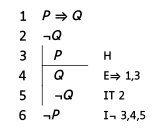
\includegraphics[width=0.4\linewidth]{files/fitch-b1b30d3bae99cd633d830976f12fffdb.svg}
\end{figure}

The sub-derivation (lines 3--5) discharges the hypothesis $P$: assuming $P$,
[$\Rightarrow$-elimination] on lines 1 and 3 gives $Q$, while line 2 reiterates
$¬ Q$. The contradiction lets us introduce $¬ P$ ($¬$-introduction over
lines 3, 4, 5).

In Lean this is theorem \texttt{T55}, where \texttt{¬P} is definitionally \texttt{P \rightarrow False},\footnote{This is the standard definition in Lean's core library: \texttt{Not p} unfolds to \texttt{p \rightarrow False},
so a proof of \texttt{¬P} is exactly a function turning a proof of \texttt{P} into a proof of \texttt{False}.} so the
whole proof is just function composition:

\begin{verbatim}
theorem T55 (h1 : P \rightarrow Q) (h2 : ¬Q) : ¬P :=
  (h2 ∘ h1)
\end{verbatim}

\subsubsection{Conjunction introduction. $P,\ P \Rightarrow Q ⊢ P \wedge Q$}

Theorem \texttt{T51} builds the pair \texttt{⟨proof of P, proof of Q⟩} directly, using the
anonymous-constructor notation \texttt{⟨\_, \_⟩}:

\begin{verbatim}
theorem T51 (h1 : P) (h2 : P \rightarrow Q) : P ∧ Q :=
  ⟨h1, h2 h1⟩
\end{verbatim}

\section{Linear Algebra}

\subsection{Linear algebra}

A scratch chapter for linear-algebra notes --- enough structure to flesh out later, and
enough variety (numbered equations, a table, admonitions, and interleaved Lean) to show
the book template in action. The runnable code lives in
\href{/LinearAlgebra-21b7e76089afe77d1ab624eef2fc49b2.lean}{\texttt{LearningLean/LinearAlgebra.lean}}.

\begin{framed}
\textbf{Note}\\
This chapter is a work in progress. Sections marked \textbf{To flesh out} are placeholders.
\end{framed}

\subsubsection{Vectors}

A vector in $\R^n$ is an ordered list of $n$ real numbers. We write column vectors as
$\vec{u} = (u_1, \dots, u_n)$ with each $u_i \in \R$.

The \textbf{dot product} of $\vec{u}, \vec{v} \in \R^n$ is the scalar

\begin{equation}
\label{eq-dot}
\vec{u} \cdot \vec{v} = \sum_{i=1}^{n} u_i\, v_i .
\end{equation}

For a concrete computation, take $\vec{u} = (1, 2, 3)$ and $\vec{v} = (4, 5, 6)$. Then by
equation (\ref{eq-dot}),

\begin{equation}
\vec{u} \cdot \vec{v} = 1\cdot 4 + 2\cdot 5 + 3\cdot 6 = 32 .
\end{equation}

In Lean, a vector is a function \texttt{Fin n \rightarrow ℝ}, and \texttt{![\dots]} is notation for one. The dot product and
the matrix operations below follow the spellings used in Mathlib \citep{mathlib2020}:\footnote{Mathlib writes the dot product as \texttt{⬝ᵥ} (\texttt{{\textbackslash}cdotv}) rather than reusing \texttt{·}, to keep
it distinct from scalar multiplication.}

\begin{verbatim}
def u : Fin 3 \rightarrow ℝ := ![1, 2, 3]
def v : Fin 3 \rightarrow ℝ := ![4, 5, 6]

#check u ⬝ᵥ v      - - `⬝ᵥ` is Mathlib's dot product, of type ℝ
\end{verbatim}

\subsubsection{Matrices}

An $m \times n$ matrix $A \in \R^{m \times n}$ is a rectangular array of scalars. For example,

\begin{equation}
A = \begin{bmatrix} 1 & 2 \\ 3 & 4 \end{bmatrix} \in \R^{2 \times 2}.
\end{equation}

The \textbf{matrix--vector product} $A\vec{x}$ takes a vector $\vec{x} \in \R^n$ to a vector in
$\R^m$. With $\vec{x} = (5, 6)$:

\begin{equation}
A\vec{x}
= \begin{bmatrix} 1 & 2 \\ 3 & 4 \end{bmatrix}\begin{bmatrix} 5 \\ 6 \end{bmatrix}
= \begin{bmatrix} 1\cdot 5 + 2\cdot 6 \\ 3\cdot 5 + 4\cdot 6 \end{bmatrix}
= \begin{bmatrix} 17 \\ 39 \end{bmatrix}.
\end{equation}

A few operations and their Mathlib spellings:

\bigskip\noindent
\begin{tabular}{p{\dimexpr 0.333\linewidth-2\tabcolsep}p{\dimexpr 0.333\linewidth-2\tabcolsep}p{\dimexpr 0.333\linewidth-2\tabcolsep}}
\toprule
Operation & Math & Lean / Mathlib \\
\hline
Dot product & $\vec{u} \cdot \vec{v}$ & \texttt{u ⬝ᵥ v} \\
Matrix--vector product & $A\vec{x}$ & \texttt{A *ᵥ x} \\
Matrix product & $AB$ & \texttt{A * B} \\
Transpose & $A^\top$ & \texttt{Aᵀ} \\
\bottomrule
\end{tabular}

\bigskip

\begin{verbatim}
def A : Matrix (Fin 2) (Fin 2) ℝ := !![1, 2; 3, 4]

#check A *ᵥ ![5, 6]   - - matrix -vector product, of type `Fin 2 \rightarrow ℝ`
\end{verbatim}

\subsubsection{Linear maps}

A \textbf{linear map} $T : \R^n \to \R^m$ is a function satisfying
$T(\alpha\vec{u} + \vec{v}) = \alpha\,T(\vec{u}) + T(\vec{v})$ for all scalars $\alpha$ and
vectors $\vec{u}, \vec{v}$. Every such map is represented by a matrix, and matrix
multiplication corresponds to composition of the maps.

\begin{framed}
\textbf{Note}\\
\textbf{To flesh out:} state and prove that \texttt{Matrix.mulVec A} is a \texttt{LinearMap}, and connect it to
\texttt{Matrix.toLin}.
\end{framed}

\subsubsection{A worked computation}

\textbf{To flesh out.} A step-by-step example --- e.g. solving $A\vec{x} = \vec{b}$ by row
reduction --- narrated alongside the corresponding Lean definitions, so the computation and its
formalization sit side by side.

\subsubsection{Exercises}

\begin{framed}
\textbf{Note}\\
\textbf{To flesh out.} Add exercises here, e.g.:

\begin{enumerate}
\item Show the dot product is symmetric: $\vec{u} \cdot \vec{v} = \vec{v} \cdot \vec{u}$.
\item Prove $(A^\top)^\top = A$ in Lean using \texttt{Matrix.transpose\_transpose}.
\end{enumerate}
\end{framed}




\bibliography{main.bib}
\end{document}
